\subsection{Fiesta: cambio de cara, caricatura y fusión}
\label{sec:fiesta}

Fiesta es un grupo nuevo de la interfaz, entre \emph{Juegos} y \emph{Mis looks}, de color rosado. Tiene tres herramientas pensadas para usar entre varias personas frente a la cámara:
\begin{itemize}
  \item \textbf{cambio de cara}: cada persona aparece con la cara de otra;
  \item \textbf{caricatura}: seis efectos que deforman los rasgos;
  \item \textbf{fusión}: un \emph{morphing} entre dos caras; el cuadro del medio es ``el hijo'' de los dos.
\end{itemize}
Las tres usan la misma maquinaria (\archivo{faces/}): una malla de 468 puntos por cara, una triangulación fija y un \emph{warp} afín por triángulo con mapeo inverso. La figura~\ref{fig:diag-fiesta} resume el proceso.

\begin{figure}[ht]
  \centering
  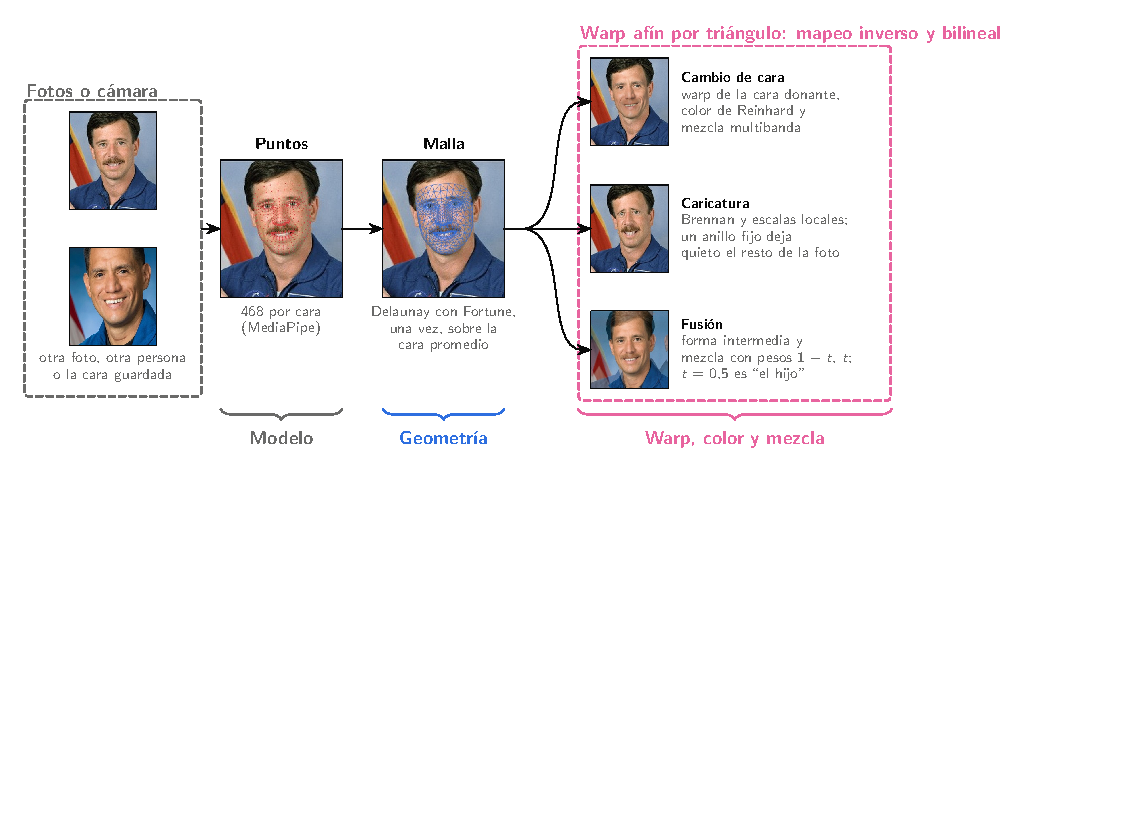
\includegraphics[width=\linewidth]{diagrama_fiesta.pdf}
  \caption{Pipeline de Fiesta: puntos de cada cara, malla con topología fija y un mismo \emph{warp} afín por triángulo para las tres herramientas.}
  \label{fig:diag-fiesta}
\end{figure}

\subsubsection{Maquinaria común}

\textbf{Puntos.} \texttt{FaceMeshes} (\archivo{faces/mesh.py}) corre el \emph{Face Landmarker} de MediaPipe con varias caras: en fotos (modo \texttt{IMAGE}) hasta 4 caras y en la cámara (modo \texttt{VIDEO}, que sigue la cara entre cuadros) hasta 3. De cada cara se usan los 468 puntos de la malla, sin los 10 del iris, en píxeles. Las caras se ordenan de izquierda a derecha. El ancho de la cara $w$ es la distancia entre los puntos 234 y 454, los extremos de las mejillas.

\textbf{Cara promedio.} La caricatura y la triangulación necesitan una cara de referencia. \archivo{backend/training/mean_face.py} la calcula una sola vez:
\begin{enumerate}
  \item corre MediaPipe sobre fotos de CelebAMask-HQ \cite{lee2020} y se queda con 400 caras frontales: la nariz debe estar a menos del 6~\% del centro entre las mejillas;
  \item normaliza cada malla: centro en el origen y radio cuadrático medio 1;
  \item alinea todas con Procrustes generalizado \cite{gower1975}: rota cada forma $X$ hacia la media actual $\bar X$ y vuelve a promediar y normalizar, cuatro veces.
\end{enumerate}
La rotación óptima sale de una descomposición en valores singulares:
\begin{equation}
  U\Sigma V^\top = X^\top\bar X,\qquad R=UV^\top,
\end{equation}
cambiando el signo de la última columna de $U$ si $\det R<0$, para no reflejar la cara. El resultado se guarda en \archivo{app/assets/faces/mean_face.npy}: solo los $468\times2$ números del promedio, ninguna foto. Se usa así:
\begin{lstlisting}
cd backend
venv/bin/python training/mean_face.py <carpeta CelebA-HQ-img> 400
\end{lstlisting}

\textbf{Topología fija.} Los triángulos se calculan una sola vez, con nuestro Fortune (sección~\ref{sec:barba}), sobre la cara promedio, y se reutilizan para todas las caras y todos los cuadros (\texttt{face\_triangles}). Hay dos razones:
\begin{itemize}
  \item el \emph{warp} lleva cada triángulo de una malla al mismo triángulo de la otra, así que las dos mallas deben tener exactamente los mismos triángulos; triangular cada cara por separado puede dar topologías distintas;
  \item en Python, Fortune tarda unos 0{,}13~s con 488 puntos: demasiado para cada cuadro de la cámara.
\end{itemize}

\textbf{Rasterización por identificador.} El \emph{warp} de la barba prueba cada píxel con coordenadas baricéntricas. Aquí se usa otra forma de rasterizar: \texttt{triangle\_ids} (\archivo{faces/warp.py}) pinta cada triángulo con \texttt{cv2.fillConvexPoly} usando su índice como ``color'', con coordenadas en punto fijo de 1/16~px. El resultado es una imagen que dice, para cada píxel, qué triángulo lo cubre ($-1$ si ninguno).

\textbf{Afines en lote.} Para cada triángulo, con vértices $(x_i,y_i)$ en el destino y $(u_i,v_i)$ en la fuente, la afín que lleva un píxel destino a su lugar en la fuente es la matriz $M$ de $3\times2$ que cumple
\begin{equation}
  \begin{pmatrix} x_1 & y_1 & 1\\ x_2 & y_2 & 1\\ x_3 & y_3 & 1 \end{pmatrix} M =
  \begin{pmatrix} u_1 & v_1\\ u_2 & v_2\\ u_3 & v_3 \end{pmatrix},
  \qquad (u,\,v)=(x,\,y,\,1)\,M.
\end{equation}
\texttt{affine\_maps} resuelve todos los sistemas de $3\times3$ en una sola llamada a \texttt{np.linalg.solve}. Los triángulos degenerados (determinante menor que $10^{-6}$) se anulan.

\textbf{Mapeo inverso y bilineal.} \texttt{warp\_mesh} recorre los píxeles cubiertos del destino: toma la $M$ de su triángulo, calcula $(u,v)$ y lee la fuente con la interpolación bilineal propia (\texttt{\_bilinear\_sample} de \archivo{geometry/warp.py}). Como cada píxel del destino busca su valor en la fuente, no quedan huecos. Todo está vectorizado con NumPy: no hay bucles por píxel.

\subsubsection{Cambio de cara}

\texttt{paste\_face} (\archivo{faces/swap.py}) pone la cara de una persona donante sobre una persona destino:
\begin{enumerate}
  \item \textbf{Recuadro.} Se trabaja en un recuadro alrededor de la malla destino, con un margen del 25~\% de $w$.
  \item \textbf{\emph{Warp}.} La foto donante se lleva, triángulo por triángulo, desde su malla hasta la malla destino. Fuera de la malla queda la foto destino.
  \item \textbf{Color.} \texttt{match\_colors} (\archivo{faces/blend.py}) aplica primero la transferencia de Reinhard \cite{reinhard2001} en CIELAB: cada canal se lleva a la media y la desviación del destino, medidas dentro de la máscara,
  \begin{equation}
    c'=(c-\mu_s)\,\operatorname{clip}\!\left(\frac{\sigma_d}{\sigma_s},\,0{,}6,\,1{,}6\right)+\mu_d.
  \end{equation}
  El recorte evita exagerar el contraste cuando una cara tiene muy poca variación. Después corrige la luz de baja frecuencia: con $\bar L=G_\sigma(L\,\alpha)/G_\sigma(\alpha)$, la luminosidad media local dentro de la máscara, y $\sigma=w/10$,
  \begin{equation}
    L' = L\cdot\operatorname{clip}\!\left(\frac{\bar L_d+5}{\bar L_s+5},\,0{,}7,\,1{,}4\right).
  \end{equation}
  Así, si la persona destino tiene luz desde la izquierda, la cara nueva también.
  \item \textbf{Máscara.} \texttt{face\_alpha} rellena la envolvente convexa del óvalo de la cara (36 puntos), la erosiona un 4~\% de $w$ y la difumina con $\sigma=0{,}05\,w$ solo hacia adentro. La línea del pelo y el borde de la mandíbula quedan de la foto original.
  \item \textbf{Mezcla multibanda.} \texttt{pyramid\_blend} sigue a Burt y Adelson \cite{burt1983}. Se arman las pirámides laplacianas $\mathcal L_k$ de las dos imágenes y la pirámide gaussiana $\mathcal G_k$ de la máscara, con hasta 5 niveles (menos si el recuadro es chico). Cada banda se mezcla con la máscara a su misma escala,
  \begin{equation}
    B_k=\big(1-\mathcal G_k(\alpha)\big)\,\mathcal L_k(\text{destino})+\mathcal G_k(\alpha)\,\mathcal L_k(\text{cara}),
  \end{equation}
  y la imagen se reconstruye sumando las bandas de la más gruesa a la más fina. Los cambios amplios de color se mezclan en una franja ancha y el detalle fino en una angosta: no queda costura ni doble contorno.
\end{enumerate}

Hay tres formas de usarlo:
\begin{itemize}
  \item \texttt{swap\_faces}: cada cara recibe la de la persona a su derecha, de forma cíclica; con dos personas es un intercambio. Todas se leen de la foto sin modificar.
  \item \texttt{wear\_face}: todos llevan la cara guardada. \texttt{set\_source} guarda la cara más grande de una foto, recortada a un lado máximo de 720~px.
  \item Con una segunda foto, la cara más grande de esa foto se pone sobre todas las caras de la primera. Así se hizo la figura~\ref{fig:fiesta-swap}.
\end{itemize}

\subsubsection{Caricatura}

\textbf{Exagerar lo propio.} La caricatura de Brennan \cite{brennan1985} agranda lo que distingue a una cara del promedio. Sea $P$ la malla de la persona y $A$ la cara promedio ajustada a $P$ con la similitud de mínimos cuadrados de Umeyama \cite{umeyama1991}: la escala $s$, la rotación $R$ y la traslación $t$ que minimizan $\sum_i\lVert s\,m_iR+t-p_i\rVert^2$, con los puntos como vectores fila. Con los puntos centrados en las matrices $X_m$ (cara promedio) y $X_p$ (persona), $U\Sigma V^\top=X_m^\top X_p$, $D=\operatorname{diag}(1,\operatorname{sign}\det(UV^\top))$, $R=UDV^\top$ y $s=\operatorname{tr}(\Sigma D)/\lVert X_m\rVert^2$. La caricatura es
\begin{equation}
  P'=A+(1+k)\,(P-A),\qquad k=2\,a,
\end{equation}
donde $a\in[0,1]$ es la intensidad elegida. Con $a=0$ la cara no cambia, y la cara promedio no tiene nada que exagerar; las pruebas verifican ambos casos.

\textbf{Escalas locales.} Los demás efectos agrandan o achican un rasgo con centro $c$, radio $r$ y factor $f$ (\texttt{bulge}):
\begin{equation}
  p'=c+(p-c)\,\Big(1+(f-1)\,S\big(1-\lVert p-c\rVert/r\big)\Big),\qquad S(x)=x^2(3-2x),\ x\in[0,1].
\end{equation}
El factor se aplica completo en el centro y se desvanece hasta el radio con un \emph{smoothstep}, así la piel alrededor se estira sin quiebres. El radio de un rasgo es $\max(1{,}4\cdot\text{tamaño},\ 0{,}14\,w)$, con el tamaño igual al lado mayor de su rectángulo envolvente; el de la cara entera es $1{,}2\,w$. La tabla~\ref{tab:caricaturas} da los seis efectos.

\begin{table}[ht]
\centering
\small
\begin{tabularx}{\linewidth}{@{}l l X@{}}
\toprule
En la interfaz & Clave & Deformación (con intensidad $a$) \\
\midrule
Caricatura & \texttt{caricature} & Brennan con $k=2a$. \\
Ojotes & \texttt{eyes} & Ojos $\times(1+0{,}9a)$. \\
Narizón & \texttt{nose} & Nariz $\times(1+1{,}0a)$. \\
Cachetón & \texttt{big-head} & Cara $\times(1+0{,}6a)$, ojos $\times(1+0{,}3a)$. \\
Carita & \texttt{tiny-face} & Cara $\times(1-0{,}4a)$. \\
Alien & \texttt{alien} & Ojos $\times(1+1{,}1a)$, boca $\times(1-0{,}45a)$, mentón $\times(1-0{,}35a)$, nariz $\times(1-0{,}3a)$. \\
\bottomrule
\end{tabularx}
\caption{Efectos de caricatura.}
\label{tab:caricaturas}
\end{table}

\textbf{Anillo fijo.} Si solo se movieran los puntos de la cara, la foto se rompería en el borde de la malla. Por eso se agrega un anillo de 28 puntos fijos sobre una elipse con centro en el óvalo de la cara y semiejes de 1{,}9 veces la semiextensión del óvalo (\texttt{ring}). Los puntos del anillo están en el mismo lugar en la malla original y en la deformada: los triángulos entre la cara y el anillo se estiran, y fuera del anillo nada se mueve. La malla con el anillo también se triangula una sola vez sobre la cara promedio. El \emph{warp} usa la malla deformada como destino y la original como fuente: cada píxel de la cara nueva lee dónde estaba antes. Se aplica a todas las caras de la foto. La figura~\ref{fig:fiesta-caricatura} muestra los seis efectos y la malla con el anillo.

\begin{figure}[ht]
  \centering
  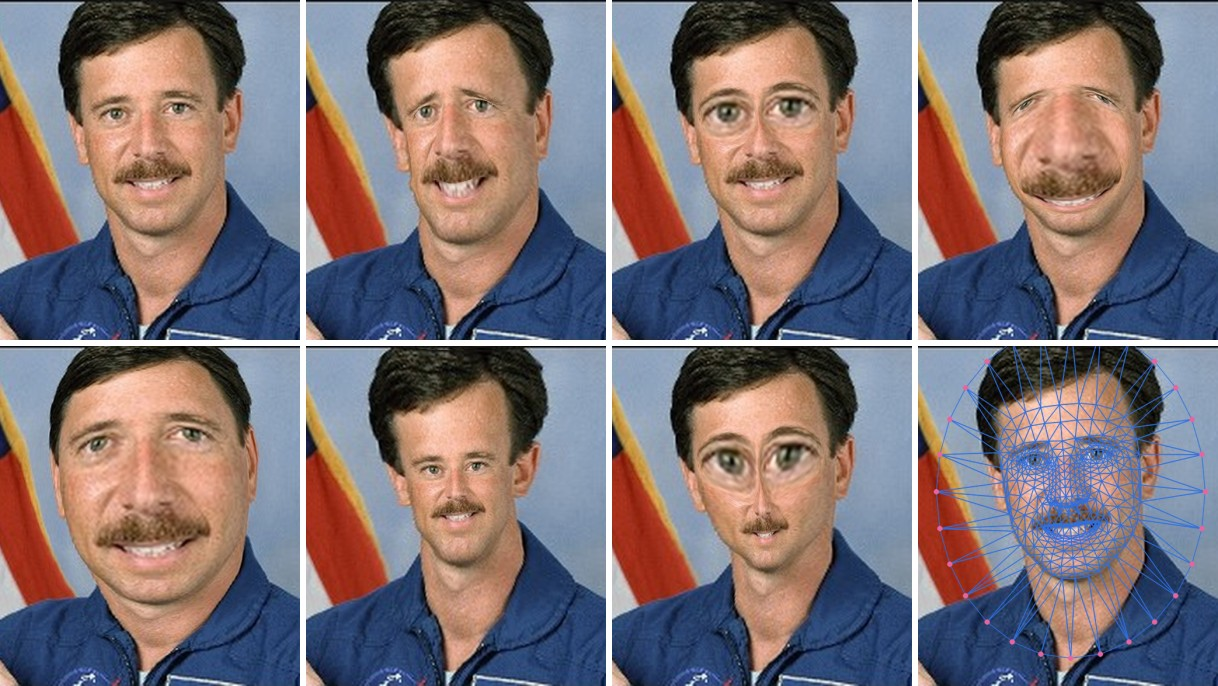
\includegraphics[width=\linewidth]{fiesta_caricatura.jpg}
  \caption{Caricaturas con intensidad 1 sobre un retrato de dominio público de la NASA. Arriba: original, Caricatura, Ojotes y Narizón. Abajo: Cachetón, Carita, Alien y la malla con el anillo de 28 puntos fijos (rosado).}
  \label{fig:fiesta-caricatura}
\end{figure}

\subsubsection{Fusión}

La fusión (\archivo{faces/morph.py}) es un \emph{morphing} clásico \cite{beier1992,wolberg1998}:
\begin{enumerate}
  \item cada cara se recorta a un cuadrado de 480~px, escalado para que el ancho de la cara sea el lado dividido por 2{,}1;
  \item la segunda cara se alinea a la primera con una similitud (\texttt{cv2.estimateAffinePartial2D} sobre los 468 puntos);
  \item cada conjunto de puntos tiene los 468 de la cara, un anillo de 20 puntos a 1{,}5 veces el óvalo y 16 puntos en el borde del cuadro, para que la malla cubra todo el cuadrado;
  \item se triangula con Fortune la forma promedio de las dos, $(A+B)/2$;
  \item para 13 valores de $t$ entre 0 y 1, las dos fotos se deforman a la forma intermedia y se mezclan:
  \begin{equation}
    S_t=(1-t)\,A+t\,B,\qquad I_t=(1-t)\,W_A(S_t)+t\,W_B(S_t),
  \end{equation}
  donde $W_A(S_t)$ es la foto de $A$ llevada con el \emph{warp} a la forma $S_t$.
\end{enumerate}
El cuadro $t=0{,}5$ tiene la forma promedio y los dos colores a medias: es ``el hijo'' de los dos. En la interfaz, un deslizador recorre los cuadros, ``Animar'' va y vuelve con una curva coseno (3{,}2~s por ciclo) y el nombre del hijo une la primera mitad del primer nombre con la segunda mitad del segundo (Kalos y Gianpier dan Kalpier). La figura~\ref{fig:fiesta-fusion} muestra cinco cuadros.

\subsubsection{En vivo, tiempos y API}

En vivo, el navegador envía cada cuadro de la cámara, reducido a 640~px de ancho, y el detector en modo \texttt{VIDEO} sigue las caras entre cuadros. \texttt{FaceStudio} (\archivo{faces/session.py}) guarda el detector de fotos, el de la cámara y la cara guardada. Medido en un Mac con chip M, solo CPU, sobre un cuadro de $640\times360$ con dos caras:
\begin{itemize}
  \item detección de las dos mallas: 12~ms;
  \item cambio de cara: 44~ms;
  \item caricatura: 49~ms.
\end{itemize}
Eso da unos 15 cuadros por segundo en el servidor. En fotos, el cambio de dos caras tarda entre 0{,}2 y 0{,}4~s según el tamaño de la foto, y la caricatura entre 0{,}05 y 0{,}15~s. Es rápido porque la topología no se recalcula, la rasterización la hace \texttt{fillConvexPoly} en C, las afines se resuelven en lote y solo se procesa el recuadro de cada cara. La fusión de 13 cuadros tarda unos 1{,}5~s: cada cuadro deforma dos imágenes completas de $480\times480$, y el muestreo bilineal de esos 26 \emph{warps} se lleva casi todo el tiempo.

\begin{table}[ht]
\centering
\small
\begin{tabularx}{\linewidth}{@{}l X@{}}
\toprule
\emph{Endpoint} & Uso \\
\midrule
\texttt{POST /api/faces/source} & Campo \texttt{image}. Guarda la cara más grande como ``la cara que se ponen'' y devuelve su recorte (JPEG). \\
\texttt{POST /api/faces/photo} & Campos \texttt{image}, \texttt{other} (opcional), \texttt{mode} (\texttt{swap}, \texttt{wear} o \texttt{caricature}), \texttt{preset} y \texttt{amount} (0 a 1). Devuelve un PNG y, en la cabecera \texttt{X-Faces}, cuántas caras vio. Con \texttt{other}, pone la cara de la segunda foto sobre la primera. \\
\texttt{POST /api/faces/live} & Un cuadro de la cámara (\texttt{image}, \texttt{mode}, \texttt{preset}, \texttt{amount}), reducido a 640~px. Devuelve JPEG y \texttt{X-Faces}. \\
\texttt{POST /api/faces/fusion} & Campos \texttt{image}, \texttt{other} (opcional) y \texttt{steps} (3 a 25). Devuelve JSON con los cuadros. Sin \texttt{other}, usa las dos caras más grandes de la foto, de izquierda a derecha. \\
\bottomrule
\end{tabularx}
\caption{\emph{Endpoints} de Fiesta.}
\label{tab:api-fiesta}
\end{table}

\textbf{Interfaz.} \archivo{frontend/js/fiesta.js} tiene tres pestañas. En \emph{Cambio de cara} se elige ``Entre ustedes'' (dos o más personas frente a la cámara) o ``Una cara para todos'': la cara guardada se toma de la cámara con una cuenta regresiva de 3~s, de una foto subida o del retrato de un astronauta. \emph{Caricatura} ofrece los seis efectos con su intensidad, en vivo o sobre una foto, y deforma todas las caras a la vez. \emph{Fusión} toma una foto de los dos juntos (con cuenta regresiva) o dos fotos.

\textbf{Pruebas.} \archivo{backend/tests/test_faces.py} tiene 19 pruebas. Verifican, entre otras cosas, que la cara promedio está normalizada, que los triángulos cubren los 468 puntos, que \texttt{affine\_maps} recupera una afín conocida, que el \emph{warp} con la misma malla es la identidad, que la mezcla multibanda respeta la máscara, que \texttt{bulge} solo mueve los puntos dentro de su radio, que Umeyama devuelve la cara promedio a su lugar, que la caricatura con intensidad 0 no cambia la foto, y los \emph{endpoints}: el intercambio entre dos personas cambia solo las dos caras, la caricatura deja quietas las esquinas de la foto y sin cara la API responde 422.
